\documentclass[11pt]{article}
% Shared preamble for manuscripts-v2 papers. Load with % Shared preamble for manuscripts-v2 papers. Load with % Shared preamble for manuscripts-v2 papers. Load with \input{../common/preamble.tex}
% immediately after \documentclass[11pt]{article}.
\ifdefined\pdftrailerid\pdftrailerid{}\fi
\usepackage[T1]{fontenc}
\usepackage{lmodern}
\usepackage[letterpaper,margin=1.02in]{geometry}
\usepackage{amsmath,amssymb,amsthm,mathtools,booktabs,array,microtype,enumitem}
\usepackage{tikz}
\usepackage{xurl}
\usepackage[colorlinks=true,allcolors=bluegreen]{hyperref}
\definecolor{bluegreen}{RGB}{22,83,91}
\usepackage[capitalize,nameinlink]{cleveref}

\theoremstyle{plain}
\newtheorem{theorem}{Theorem}[section]
\newtheorem{lemma}[theorem]{Lemma}
\newtheorem{proposition}[theorem]{Proposition}
\newtheorem{corollary}[theorem]{Corollary}
\newtheorem{conjecture}[theorem]{Conjecture}
\newtheorem*{theorem*}{Theorem}
\newtheorem{maintheorem}{Theorem}
\renewcommand{\themaintheorem}{\Alph{maintheorem}}
\theoremstyle{definition}
\newtheorem{definition}[theorem]{Definition}
\newtheorem{example}[theorem]{Example}
\newtheorem{question}[theorem]{Question}
\theoremstyle{remark}
\newtheorem{remark}[theorem]{Remark}
\crefname{maintheorem}{Theorem}{Theorems}
\crefname{conjecture}{Conjecture}{Conjectures}
\crefname{question}{Question}{Questions}
\crefname{example}{Example}{Examples}

\newcommand{\R}{\mathbb R}
\newcommand{\Q}{\mathbb Q}
\newcommand{\Z}{\mathbb Z}
\newcommand{\N}{\mathbb N}
\newcommand{\T}{\mathbb T}
\newcommand{\C}{\mathbb C}
\DeclareMathOperator{\den}{den}
\newcommand{\e}{\mathrm e}

% Immutable Lean source links at research-checkpoint-18.
\newcommand{\leancommit}{e4809cf561573aef588e6ffc491a35cdb79fd9ec}
\newcommand{\leanbase}{https://github.com/eldernos/MathematicsResearch/blob/\leancommit}
% \lean{File}{line}{label}: link to NormalityChecker/File.lean#Lline at the pinned commit.
\newcommand{\lean}[3]{\href{\leanbase/NormalityChecker/#1.lean\#L#2}{#3}}
% \repo{path}{label}: link to any repository path at the pinned commit.
\newcommand{\repo}[2]{\href{https://github.com/eldernos/MathematicsResearch/tree/\leancommit/#1}{#2}}

% Evidence labels (see papers/WAVE2-CONTRACT.md).
\newcommand{\evidence}[1]{\textup{[\emph{#1}]}}

\setlength{\emergencystretch}{1.5em}
\raggedbottom

% immediately after \documentclass[11pt]{article}.
\ifdefined\pdftrailerid\pdftrailerid{}\fi
\usepackage[T1]{fontenc}
\usepackage{lmodern}
\usepackage[letterpaper,margin=1.02in]{geometry}
\usepackage{amsmath,amssymb,amsthm,mathtools,booktabs,array,microtype,enumitem}
\usepackage{tikz}
\usepackage{xurl}
\usepackage[colorlinks=true,allcolors=bluegreen]{hyperref}
\definecolor{bluegreen}{RGB}{22,83,91}
\usepackage[capitalize,nameinlink]{cleveref}

\theoremstyle{plain}
\newtheorem{theorem}{Theorem}[section]
\newtheorem{lemma}[theorem]{Lemma}
\newtheorem{proposition}[theorem]{Proposition}
\newtheorem{corollary}[theorem]{Corollary}
\newtheorem{conjecture}[theorem]{Conjecture}
\newtheorem*{theorem*}{Theorem}
\newtheorem{maintheorem}{Theorem}
\renewcommand{\themaintheorem}{\Alph{maintheorem}}
\theoremstyle{definition}
\newtheorem{definition}[theorem]{Definition}
\newtheorem{example}[theorem]{Example}
\newtheorem{question}[theorem]{Question}
\theoremstyle{remark}
\newtheorem{remark}[theorem]{Remark}
\crefname{maintheorem}{Theorem}{Theorems}
\crefname{conjecture}{Conjecture}{Conjectures}
\crefname{question}{Question}{Questions}
\crefname{example}{Example}{Examples}

\newcommand{\R}{\mathbb R}
\newcommand{\Q}{\mathbb Q}
\newcommand{\Z}{\mathbb Z}
\newcommand{\N}{\mathbb N}
\newcommand{\T}{\mathbb T}
\newcommand{\C}{\mathbb C}
\DeclareMathOperator{\den}{den}
\newcommand{\e}{\mathrm e}

% Immutable Lean source links at research-checkpoint-18.
\newcommand{\leancommit}{e4809cf561573aef588e6ffc491a35cdb79fd9ec}
\newcommand{\leanbase}{https://github.com/eldernos/MathematicsResearch/blob/\leancommit}
% \lean{File}{line}{label}: link to NormalityChecker/File.lean#Lline at the pinned commit.
\newcommand{\lean}[3]{\href{\leanbase/NormalityChecker/#1.lean\#L#2}{#3}}
% \repo{path}{label}: link to any repository path at the pinned commit.
\newcommand{\repo}[2]{\href{https://github.com/eldernos/MathematicsResearch/tree/\leancommit/#1}{#2}}

% Evidence labels (see papers/WAVE2-CONTRACT.md).
\newcommand{\evidence}[1]{\textup{[\emph{#1}]}}

\setlength{\emergencystretch}{1.5em}
\raggedbottom

% immediately after \documentclass[11pt]{article}.
\ifdefined\pdftrailerid\pdftrailerid{}\fi
\usepackage[T1]{fontenc}
\usepackage{lmodern}
\usepackage[letterpaper,margin=1.02in]{geometry}
\usepackage{amsmath,amssymb,amsthm,mathtools,booktabs,array,microtype,enumitem}
\usepackage{tikz}
\usepackage{xurl}
\usepackage[colorlinks=true,allcolors=bluegreen]{hyperref}
\definecolor{bluegreen}{RGB}{22,83,91}
\usepackage[capitalize,nameinlink]{cleveref}

\theoremstyle{plain}
\newtheorem{theorem}{Theorem}[section]
\newtheorem{lemma}[theorem]{Lemma}
\newtheorem{proposition}[theorem]{Proposition}
\newtheorem{corollary}[theorem]{Corollary}
\newtheorem{conjecture}[theorem]{Conjecture}
\newtheorem*{theorem*}{Theorem}
\newtheorem{maintheorem}{Theorem}
\renewcommand{\themaintheorem}{\Alph{maintheorem}}
\theoremstyle{definition}
\newtheorem{definition}[theorem]{Definition}
\newtheorem{example}[theorem]{Example}
\newtheorem{question}[theorem]{Question}
\theoremstyle{remark}
\newtheorem{remark}[theorem]{Remark}
\crefname{maintheorem}{Theorem}{Theorems}
\crefname{conjecture}{Conjecture}{Conjectures}
\crefname{question}{Question}{Questions}
\crefname{example}{Example}{Examples}

\newcommand{\R}{\mathbb R}
\newcommand{\Q}{\mathbb Q}
\newcommand{\Z}{\mathbb Z}
\newcommand{\N}{\mathbb N}
\newcommand{\T}{\mathbb T}
\newcommand{\C}{\mathbb C}
\DeclareMathOperator{\den}{den}
\newcommand{\e}{\mathrm e}

% Immutable Lean source links at research-checkpoint-18.
\newcommand{\leancommit}{e4809cf561573aef588e6ffc491a35cdb79fd9ec}
\newcommand{\leanbase}{https://github.com/eldernos/MathematicsResearch/blob/\leancommit}
% \lean{File}{line}{label}: link to NormalityChecker/File.lean#Lline at the pinned commit.
\newcommand{\lean}[3]{\href{\leanbase/NormalityChecker/#1.lean\#L#2}{#3}}
% \repo{path}{label}: link to any repository path at the pinned commit.
\newcommand{\repo}[2]{\href{https://github.com/eldernos/MathematicsResearch/tree/\leancommit/#1}{#2}}

% Evidence labels (see papers/WAVE2-CONTRACT.md).
\newcommand{\evidence}[1]{\textup{[\emph{#1}]}}

\setlength{\emergencystretch}{1.5em}
\raggedbottom

% Author information approved by the repository owner on 2026-11-25:
%   name: Christopher Anderson; designation: Independent Researcher.
% No academic affiliation, ORCID or personal contact details have been supplied.
% Do not add any that the owner has not approved.
\newcommand{\OwnerAuthor}{Christopher Anderson}
\newcommand{\OwnerAffiliation}{Independent Researcher}
\newcommand{\OwnerContact}{Corrections and comments: \url{https://github.com/eldernos/MathematicsResearch/issues}}
\newcommand{\ReleaseLabel}{manuscripts-v2.0.0}
\newcommand{\LicenseLine}{\copyright\ 2026 Christopher Anderson. Licensed under \href{https://creativecommons.org/licenses/by/4.0/}{CC BY 4.0}.}
% \makebyline{version}{date}: centred author block used under the title.
\newcommand{\makebyline}[2]{%
  {\large \OwnerAuthor\par}%
  \ifx\OwnerAffiliation\empty\else{\small \OwnerAffiliation\par}\fi
  \vspace{0.3em}
  {\small Version #1 \enspace$\cdot$\enspace #2 \enspace$\cdot$\enspace \ReleaseLabel\par}%
  {\footnotesize \OwnerContact\par}%
  {\footnotesize \LicenseLine\par}%
  \hypersetup{pdfauthor={\OwnerAuthor}}}

\hypersetup{pdftitle={Normality of localized logarithms and polylogarithms on finite prime supports}}
\newcommand{\vol}{\lambda}
\newcommand{\Dinf}{D_{\infty}}
\newcommand{\fract}[1]{\{#1\}}
\newcommand{\decl}[3]{\lean{#1}{#2}{\texttt{#3}}}
\setlength{\emergencystretch}{3em}
\title{Normality of localized logarithms and polylogarithms\\on finite prime supports}
\author{}
\date{}
\begin{document}
\maketitle
\begin{center}\makebyline{2.0}{25 November 2026}\end{center}
\begin{abstract}
Let $M(S)$ be the set of positive integers whose prime factors lie in a finite set $S$ of primes. For integers $b\ge2$ and $s\ge1$, the series $\sum_{m\in M(S)}m^{-s}b^{-m}$ has base-$b$ interval discrepancy tending to $0$ if some $p\in S$ does not divide $b$, and to $1$ otherwise. For a nonzero rational polynomial $P$, the series with numerator $P(m)$ is normal exactly when $P(X)/X^s$ has a pole at zero and such a prime exists. The proof shows that persistent cancellation at an off-radix prime has measure zero, by taking multiplicative differences on a logarithmic circle and separating the remaining thresholds. We also show that the shifts of the series at distinct positive orders on one support, with rational numerators nonzero at zero, are jointly equidistributed in the unit cube. For retained subsets of the support we bound the discrepancy by the missed density of retained prime-power windows, and we classify normality on a single prime-power axis. For a fixed prime, finitely many orders and a positive tolerance, a depth at which every finite certificate is below the tolerance can be computed. The main classifications and the joint theorem are verified by the Lean kernel; the proofs written here are explanatory, and priority statements are provisional.
\end{abstract}

\section{Introduction and main results}\label{sec:intro}
For a finite set $S$ of primes put $M(S)=\{m\ge1:\ p\mid m,\ p\text{ prime}\Rightarrow p\in S\}$, so that $M(\varnothing)=\{1\}$. For integers $b\ge2$ and $s\ge0$, a polynomial $P\in\Q[X]$ and a subset $A\subseteq M(S)$ write
\begin{equation}\label{eq:series}
 X_A(P,s)=\sum_{m\in A}\frac{P(m)}{m^s b^m},\qquad
 X_s=X_{M(S)}(1,s),\qquad J=\{p\in S:p\nmid b\}.
\end{equation}
Polynomial growth of the coefficients gives absolute convergence for every $A$. For $s=1$ the sum $X_1$ localizes the positive-coefficient series of $-\log(1-b^{-1})$ to the integers supported on $S$; for $s\ge1$ the sum $X_s$ localizes $\operatorname{Li}_s(b^{-1})$. Dibag introduced the localization of the logarithm at a set of primes in work on generalized Bernoulli coefficients \cite[Definitions~1.1--1.2]{dibag}.

Write $\{y\}=y-\lfloor y\rfloor$. For $0\le a<c\le1$ and $N\ge1$ put
\[
 f_N(x;[a,c))=\frac1N\#\{0\le n<N:a\le\fract{b^nx}<c\},\qquad
 D_N(x)=\sup_{a,c}|f_N(x;[a,c))-(c-a)|,
\]
and $\Dinf(x)=\limsup_{N\to\infty}D_N(x)$. A real number is \emph{normal in radix $b$} if every word of length $k\ge1$ has limiting frequency $b^{-k}$ at overlapping starting positions, with terminating expansions at radix rationals. A word of length $k$ specifies a half-open interval $[j/b^k,(j+1)/b^k)$. Convergence $D_N\to0$ implies all these frequencies. Conversely each interval is bracketed by unions of cylinders at one depth whose total length differs from its length by at most $2b^{-k}$, and the maximum error over the finitely many such unions tends to zero at each fixed $k$. Hence $x$ is normal if and only if $D_N(x)\to0$, that is, if and only if $(\{b^nx\})_{n\ge0}$ is uniformly distributed modulo one.

\subsection{Main results}
Each theorem carries one evidence label (\cref{sec:formal}). Declaration names refer to the Lean development at the pinned revision.

\begin{maintheorem}[Unsigned series on the full support]\label{thm:unsigned}
For every finite set $S$ of primes, integer $b\ge2$ and integer $s\ge1$,
\[
 \lim_{N\to\infty}D_N(X_s)=
 \begin{cases}0,&J\ne\varnothing,\\1,&J=\varnothing.\end{cases}
\]
In particular $X_s$ is normal in radix $b$ exactly when $J\ne\varnothing$. \evidence{Kernel-verified}: \decl{UnsignedNormality}{198}{unsigned\_\allowbreak{}discrepancy\_\allowbreak{}limit} and \decl{UnsignedNormality}{191}{unsigned\_\allowbreak{}finite\_\allowbreak{}support\_\allowbreak{}normal}. The statement in definitions from mathlib alone is checked in \texttt{Check.lean} (\cref{sec:formal}).
\end{maintheorem}

\begin{maintheorem}[Rational polynomial weights]\label{thm:polynomial}
Let $P\in\Q[X]\setminus\{0\}$, let $r$ be its order of vanishing at zero, and let $s\ge0$. Then $X_{M(S)}(P,s)$ is normal in radix $b$ if and only if $r<s$ and $J\ne\varnothing$. If $r\ge s$ or $J=\varnothing$, then every restriction $X_A(P,s)$, $A\subseteq M(S)$, is not normal, and there is an integer $L\ge1$ coprime to $b$ with $\liminf_N D_N(X_A(P,s))\ge1/L$. If $P\in\Z[X]$ and $r\ge s$ or $J=\varnothing$, then $D_N(X_A(P,s))\to1$ for every restriction $A$. \evidence{Kernel-verified}: \decl{FullPolynomialNormality}{15}{full\_\allowbreak{}rational\_\allowbreak{}normal\_\allowbreak{}iff}, \decl{MaskRational}{54}{rational\_\allowbreak{}boundary}, \decl{MaskGrid}{174}{integer\_\allowbreak{}mask\_\allowbreak{}maximal}.
\end{maintheorem}

\begin{maintheorem}[Joint distribution at distinct orders]\label{thm:joint}
Let $S$ be a finite set of primes, let $d\ge1$, let $s_1,\dots,s_d$ be pairwise distinct positive integers, and let $P_1,\dots,P_d\in\Q[X]$ satisfy $P_i(0)\ne0$. Put $Y_i=X_{M(S)}(P_i,s_i)$.
\begin{enumerate}[label=\textup{(\roman*)},leftmargin=2em]
\item If $J\ne\varnothing$, then for every box $\prod_i[a_i,c_i)\subseteq[0,1)^d$ the proportion of $0\le n<N$ with $\{b^nY_i\}\in[a_i,c_i)$ for every $i$ tends to $\prod_i(c_i-a_i)$. Equivalently, the vectors $(\{b^nY_1\},\dots,\{b^nY_d\})$ are uniformly distributed in $[0,1)^d$. In particular this holds for the unsigned series $X_{s_1},\dots,X_{s_d}$ on one fixed support.
\item Let $S=\{p\}$ with $p\nmid b$ and let $K\subseteq\mathbb Z_{\ge0}$ be a common set of retained exponents, so that $Y_i^K=\sum_{k\in K}P_i(p^k)p^{-ks_i}b^{-p^k}$. The conclusion of \textup{(i)} holds for $(Y_i^K)_i$ if and only if $K$ is infinite.
\item Let $b$ be odd and $2\in S$. If a common retained set $A\subseteq M(S)$ contains $2^k$ for all sufficiently large $k$, the conclusion of \textup{(i)} holds for the sums $X_A(P_i,s_i)$, with arbitrary membership of the other smooth indices.
\end{enumerate}
\evidence{Kernel-verified}: \decl{LocalizedJoint}{85}{joint\_\allowbreak{}full\_\allowbreak{}polynomial\_\allowbreak{}orders} for \textup{(i)}; \decl{LocalizedJoint}{158}{joint\_\allowbreak{}full\_\allowbreak{}orders} and \decl{LocalizedJoint}{167}{distinct\_\allowbreak{}orders\_\allowbreak{}checked} for the unsigned case; \decl{LocalizedJoint}{107}{joint\_\allowbreak{}axis\_\allowbreak{}orders\_\allowbreak{}iff} for \textup{(ii)}; \decl{LocalizedJoint}{118}{joint\_\allowbreak{}late\_\allowbreak{}twos\_\allowbreak{}orders} for \textup{(iii)}. The mathlib-only statement of \textup{(i)} is checked in \texttt{Check.lean}.
\end{maintheorem}

The unsigned case of \cref{thm:joint}(i) is Corollary 1.3 of version 1.1 of this paper, where it was a written deduction. It is now a theorem about a Lean declaration, with polynomial numerators and common masks added. The precise scope of what the kernel checks is given in \cref{sec:formal}.

\begin{maintheorem}[Retained subsets, windows and axes]\label{thm:mask}
Let $b\ge2$, let $p\in S$ be a prime with $p\nmid b$, and let $P\in\Q[X]\setminus\{0\}$ have order of vanishing $r<s$ at zero. Let $A\subseteq M(S)$, let $K=\{k\ge0:p^k\in A\}$, $W=\bigcup_{k\in K}[p^k,2p^k)\cap\Z$ and $g=\liminf_N\#(W\cap[0,N))/N$.
\begin{enumerate}[label=\textup{(\roman*)},leftmargin=2em]
\item $\Dinf(X_A(P,s))\le1-g$.
\item If the retained exponents $k_1<k_2<\cdots$ satisfy $k_{j+1}-k_j\le h$ for all large $j$, then $\Dinf\le1-1/(p^h-1)$. In particular if $A$ contains $p^k$ for all large $k$ then $\Dinf\le1-1/(p-1)$, and if moreover $p=2$ and $b$ is odd, then $X_A(P,s)$ is normal.
\item If $S=\{p\}$, then $X_A(P,s)$ is normal if and only if $K$ is infinite.
\end{enumerate}
\evidence{Lean-supported paper proof} for \textup{(i)}: the Lean step is the window bound \decl{MaskClassification}{122}{rational\_\allowbreak{}window\_\allowbreak{}bound}; the passage to $g$ is the counting argument in \cref{sec:masks}. Parts \textup{(ii)} and \textup{(iii)} are \evidence{Kernel-verified}: \decl{MaskAxis}{138}{axis\_\allowbreak{}normal\_\allowbreak{}iff}, \decl{MaskRational}{38}{rational\_\allowbreak{}pole\_\allowbreak{}bound}, \decl{MaskWindows}{107}{late\_\allowbreak{}powers\_\allowbreak{}discrepancy}, \decl{MaskWindows}{114}{normal\_\allowbreak{}of\_\allowbreak{}late\_\allowbreak{}twos}.
\end{maintheorem}

\begin{maintheorem}[A computable common depth]\label{thm:depth}
Let $p\in J$, let $S'=S\setminus\{p\}$, let $T$ be a finite set of positive orders and let $\varepsilon\in\Q_{>0}$. For $k\ge0$ let $E_s(k)$ be the set of failed cells of order $s$ at depth $k$ and $C_s(k)$ the worst-prefix certificate at that depth, both defined in \cref{sec:local}. The least $k$ with $2\#E_s(k)/p^k<\varepsilon$ for all $s\in T$ exists and is computed by finite integer arithmetic. For every $k'\ge k$ and every $s\in T$ one has $C_s(k')<\varepsilon$, hence $\Dinf(X_s)<\varepsilon$. \evidence{Kernel-verified}: \decl{LocalizedCertificateModulus}{21}{exists\_\allowbreak{}common\_\allowbreak{}depth}, \decl{LocalizedCertificateModulus}{44}{certificateModulus\_\allowbreak{}spec}.
\end{maintheorem}

\cref{thm:depth} gives a precision for the finite certificates. It does not give a cutoff $N$ in terms of which a rectangle frequency or a digit-word frequency is within $\varepsilon$ of its limit, and by \cref{prop:uniform} no such cutoff can be uniform over masks.

\begin{maintheorem}[A rate on two-generator supports]\label{thm:rate}
Let $b,q\ge2$ be integers with $q\mid b$ and let $p$ be an odd prime with $p\nmid b$. The number $X=\sum_{a,j\ge0}q^{-a}p^{-j}b^{-q^ap^j}$ is normal in radix $b$, and there are $A>0$ and $N_0$ with $D_N(X)\le A/\log\log N$ for all $N\ge N_0$. \evidence{Kernel-verified}: \decl{LocalizedDiscrepancy}{266}{discrepancy\_\allowbreak{}rate} in the definitions of the library. The constant $A$ depends on $(b,q,p)$ and is not computed.
\end{maintheorem}

\subsection{Relation to earlier and contemporaneous work}\label{sec:related}
Priority statements here are provisional. We examined the sources below; we have not located the exact statements of \cref{thm:unsigned,thm:polynomial,thm:joint,thm:mask} in them, and a failed search proves nothing about novelty. No specialist has reviewed these comparisons. Full records are in the accompanying ledger.

\emph{Singleton supports.} For $S=\{p\}$ with $p\nmid b$ and $s=1$, $X_1=b^{-1}+\alpha_{b,p}$ with $\alpha_{b,c}=\sum_{j\ge1}c^{-j}b^{-c^j}$ the Stoneham constant. Stoneham proved normality under primitive-root hypotheses \cite{stoneham}; Bailey and Crandall proved it for all coprime $b,c$ \cite[Corollary~4.9(i)]{bc}. For any infinite subset of one off-radix prime-power axis, Vandehey's Theorem~7.4 \cite{vandehey} (preprint numbering) gives normality of the unsigned series, because the denominators form a divisibility chain; Kano's general construction \cite[Theorem~1]{kano} allows varying integer numerators on Stoneham-type schedules and contains Korobov's constructions as the case of unit numerators \cite{korobov}. A recent note of Captain Sude characterizes normality of $\alpha_{b,c}$ for composite $c$ by the existence of a prime dividing $c$ and not $b$ \cite{sudeprime}; for prime $c$ this is the case $|S|=1$ of \cref{thm:unsigned}. A second public archive of Mira (7 October 2026) \cite[S07, Theorems~1.1, 1.2 and 9.1, as summarized in its result list]{mirabis} states a classification of normality, and of joint normality at mixed orders by a rank condition, for $\sum_{k\ge1}A_kp^{-sk}b^{-p^k}$ with $A_k$ rational and periodic in $k$, on the full axis of one off-radix prime and every order $s\ge1$. \cref{prop:periodic} below is, in our reading, a case of that scalar classification at $s=1$; we have not compared the form of the finite tests, and we have not checked the proofs in that archive, which states that it has had no independent audit.

\emph{Supports wholly prime to the radix.} Mira's working notes of 22 September 2026 \cite[S09, Theorem~1; see also T30]{mira} prove, by a Korobov-type argument and with the least prime of $S$ supplying an uncancelled denominator power, that $\sum_{m\in M(S)}m^{-s}b^{-m}$ is normal for every positive order when $S$ is nonempty and no prime of $S$ divides $b$. A note of Mira Cult dated 24 November 2026, which states that it consolidates the earlier archive, restates this as its Theorem~2 \cite{miracult}. Captain Sude proves the order-one case with a Lean development for the binary support $\{2,3\}$ and a paper proof for all nonempty $S$ prime to $b$, and for $b=2$ with $3\in S$ \cite[Theorems~1.1 and 5.1]{localized}; the binary $\{2,3\}$ case also carries the discrepancy bound $O(N^{-1/2}\log^3N)$ \cite[Theorem~4.1]{localized}.

\emph{Two generators, one off the radix.} Sude's later family \cite[Theorem~1]{xifamily} shows that $\sum_{m\in\{a^ic^k\}}m^{-1}b^{-m}$ is normal in radix $b$ whenever $\gcd(c,ab)=1$, with $a$ allowed to share primes with $b$, and that rational combinations over different $c$ are normal. Taking $a,c$ to be the two primes of $S$ shows that \cref{thm:unsigned} at order one on a two-prime support with an off-radix prime is already a consequence of \cite[Theorem~1]{xifamily}; their proof also extends to periodic weights depending on the exponent of $c$. The method there uses that cofactor terms with equal $p$-adic valuation lie a multiplicative factor at least $a\ge2$ apart. It does not apply directly to supports with two or more cofactor primes, where such terms can be arbitrarily close, which is the case treated by \cref{sec:null}.

\emph{What the sources examined do not state.} We have not found in them (a) at order one, supports with at least three primes of which one divides the radix, other than binary supports containing $3$, (b) the full dichotomy with the value $1$ of the limit when every support prime divides the radix, for supports with $|S|\ge2$, (c) any order $s\ge2$ on mixed supports, (d) arbitrary rational polynomial weights with the pole criterion of \cref{thm:polynomial}, (e) joint distribution at distinct orders on a support with more than one prime, or on a support containing radix primes, or with polynomial numerators, and (f) the window bounds and the axis classification of \cref{thm:mask} for signed polynomial numerators of unrestricted degree.

\emph{Joint results.} Mira's note \cite[S09, Theorem~2]{mira} and its restatement \cite[Theorem~1]{miracult} prove that, for finitely many distinct pairs $(p_i,s_i)$ with $p_i\nmid b$ prime, the vector of the values $\sum_{k\ge0}p_i^{-s_ik}b^{-p_i^k}$ is uniformly distributed, so that every nontrivial rational combination is normal. With $S=\{p\}$, \cref{thm:joint}(i) recovers the case of a single prime and several orders, with rational combinations arising from the Laurent numerators. \Cref{thm:joint} does not treat the joint distribution of the series on two different one-prime supports, which Mira's theorem does, and it covers fixed supports with several primes, radix primes in $S$, and polynomial numerators, which that theorem does not. The functional equation $F(z)-p^{-1}F(z^p)=z$ shows that the common argument $1/b$ cannot be varied \cite{mira,miracult}.

\emph{Methods.} Normality of rational orbits between insertions uses Vandehey's fixed-support exponential-sum estimate \cite[Corollary~1.2]{vandehey}; Section~\ref{sec:null} uses a recurrence argument on the logarithmic circle and a $p$-adic separation of finitely many geometric rays. We have not located these two steps in the literature on Stoneham-type numbers \cite{bc,kano,korobov,vandehey}; this is a statement about our search only. Bourgain's estimate for exponential sums over multiplicative subgroups modulo an arbitrary integer \cite[Theorem~8.28, as restated in Theorem~2.5 of \cite{vandehey}]{bourgain} does not require a fixed finite prime support. We have not examined whether it could replace the fixed-support input of \cref{lem:transfer}; the constants in \cref{thm:unsigned} are in any case not uniform in $S$.

\emph{Quantitative statements.} For $S=\{p\}$ and $s=1$ the number $X_1$ is a rational translate of a Stoneham constant, and Bailey and Crandall give a discrepancy bound of order $N^{-1/2}\log^2N$ for their rational-orbit sequence with $m_i=c^i$, $n_i=i$ \cite[p.~535]{bc}; transferring this to the ordinary orbit is a further step not carried out here. For supports with two or more primes the proof of \cref{thm:null} is qualitative and gives no modulus for the convergence of the failed widths, so \cref{thm:unsigned,thm:polynomial} carry no rate, except in the situation of \cref{thm:rate} and for the explicit binary $\{2,3\}$ case of Sude \cite{localized}. No uniformity in $S$ is asserted. In the unrestricted logarithm every positive integer is an insertion, whereas the count of exceptional digit positions below uses the sparsity of $M(S)$ for fixed $S$. In particular these theorems do not decide binary normality of $\log2$.

\subsection{Examples}
Figure~\ref{fig:matrix} records instances of \cref{thm:unsigned}. At $b=10$ and $S=\{2,3,5\}$ the single prime $3$ suffices in every positive order although both radix primes lie in $S$. The box $[\tfrac14,\tfrac12)\times[0,1)\times[\tfrac12,\tfrac34)$ is visited with limiting frequency $\tfrac1{16}$ by the shifts of $(X_4,X_1,X_3)$ for this $b$ and $S$ (\cref{thm:joint}(i)). A repeated order would give identical coordinates, and the box $[0,\tfrac12)\times[\tfrac12,1)$ would have frequency zero at every cutoff although its area is $\tfrac14$.

\begin{figure}[ht]
\centering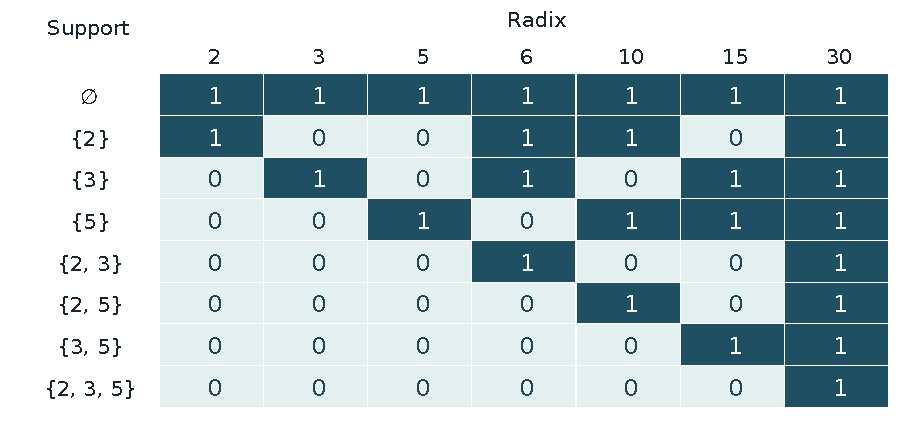
\includegraphics[width=.77\linewidth]{figures/classification.pdf}
\caption{Limit of the unsigned interval discrepancy for the indicated full supports and radices, at each integer order $s\ge1$. Zero denotes normality. Each entry follows from divisibility by the radix (\cref{thm:unsigned}).}\label{fig:matrix}
\end{figure}

\section{Rational orbits between insertions}\label{sec:orbits}
Write $a_m=P(m)/m^s$ for $m\in A$ and $a_m=0$ elsewhere, and set $R_n=\sum_{1\le m\le n}a_mb^{n-m}$. For the unsigned full support use $R_{s,n}$. If $(n,n+i]$ contains no index of $A$ then $R_{n+i}=b^iR_n$. In the unsigned case
\begin{equation}\label{eq:tail}
 0\le b^nX_s-R_{s,n}\le (n+1)^{-s}/(b-1).
\end{equation}
For a polynomial numerator the shifted tail can grow immediately before an insertion.

\begin{lemma}[Transfer on intervals without insertions]\label{lem:transfer}
Fix $S$, $b$, $P$, $s$ and $A\subseteq M(S)$. At each cutoff $N$ one can discard $o(N)$ positions, uniformly in $A$, and partition the remaining ones into blocks $[u,u+B)$ with $B=\lfloor\sqrt N\rfloor$ such that the following hold uniformly as $N\to\infty$.
\begin{enumerate}[label=\textup{(\arabic*)},leftmargin=2em]
\item $R_{u+i}=b^iR_u$ for $0\le i<B$, and $b^{u+i}X_A(P,s)-R_{u+i}=o(1)$.
\item The reduced denominator $q_u=\den(R_u)$ has prime factors in a fixed finite set of primes prime to $b$, and $q_u\le B^C$ for a fixed $C$.
\item For every $\varepsilon>0$ there are $N_0,Q_0$ such that on every retained block with $N\ge N_0$ and $q_u\ge Q_0$ the discrepancy of its $B$ shifts is at most $\varepsilon$.
\end{enumerate}
\evidence{Paper proof}. External input: \cite[Corollary~1.2]{vandehey}, exponential sums $\sum_{t<L}\exp(2\pi i\,ab^t/q)$ for $q$ supported on a fixed finite set of primes prime to $b$ and $L\ge q^{\epsilon}$. The Lean development contains an independently formalized fixed-support estimate, \decl{SmoothOrbit}{207}{fixed\_\allowbreak{}support\_\allowbreak{}orbit\_\allowbreak{}estimate}.
\end{lemma}
\begin{proof}
The number of smooth integers up to $Y$ is at most $(1+\lfloor\log_2Y\rfloor)^{|S|}$, by their exponent vectors. Partition $[0,N)$ at multiples of $B$. Omit the initial block, the final remainder and every block with a smooth index in $[u-B,u+2B]$. Each smooth index up to $N+2B$ removes at most four blocks, so the discarded length is $O(B(1+\log N)^{|S|})=o(N)$. With $|a_m|\le K(m+1)^e$ the error at a retained position $n=u+i$ is bounded by
\[
 K(n+B+2)^eb^{-B-1}\sum_{j\ge0}(1+j)^eb^{-j}=o(1),
\]
because the next $B$ positions contain no index of $A$. This gives (1).

Let $c=\prod_{p\in J}p$ and $H=\lceil\log_2(N+2B)\rceil$. In every contributing $m\le u$ each prime exponent is at most $H$, and the primes of $S$ are those of $c$ together with primes dividing $b$, so $m^s$ divides $b^{sH}c^{sH}$. Write the common coefficient denominator $D=D_bD_0$ with $D_b\mid b^\ell$ and $(D_0,b)=1$. Since $u-m\ge B>sH+\ell$ for large $N$, the denominator of each shifted summand divides $D_0c^{sH}$. This is a common denominator with the asserted support, and it is at most $B^C$ for a fixed $C$, which gives (2).

For a fixed integer $h\ne0$, $\den(hR_u)\ge q_u/|h|$. Let $q=\den(hR_u)$. By the cited estimate, $|\sum_{i<B}\exp(2\pi i\,hb^iR_u)|=o(B)$ uniformly when $q\to\infty$ and $q\le B^C$, since then $B\ge q^{1/C}$. Replacing $b^iR_u$ by $b^{u+i}X_A(P,s)$ changes the mean by at most $2\pi|h|$ times the uniform error of (1). Hence each nontrivial Fourier coefficient of the empirical measure of a sequence of such blocks tends to zero, and approximation by trigonometric polynomials gives weak convergence to Lebesgue measure. Testing intervals with endpoints on a fixed finite grid and bracketing an arbitrary interval between grid intervals gives uniform interval convergence. A failure of uniformity over the blocks would give a sequence of blocks contradicting that convergence.
\end{proof}

Consequently, if a class of positions forces uniformly growing denominators, every retained block meeting the class has a growing starting denominator, because $\den(R_{u+i})\mid\den(R_u)$. The discrepancy of a prefix is then at most the proportion outside these blocks plus $o(1)$. For a fixed error tolerance, the Fourier cutoff and the denominator threshold are chosen before $N$.

\section{Local moments and finite residue tests}\label{sec:local}
Fix $p\in J$ and put $T=M(S\setminus\{p\})$. Let $v_p$ be the $p$-adic valuation, with $v_p(0)=+\infty$. The Teichm\"uller lift of $b^{-1}\bmod p$ is the unique $w\in\Z_p^\times$ with $w^p=w$ and that reduction; it exists by Hensel lifting of $X^p-X$, whose derivative is a unit modulo $p$. Write $b^{-1}=w(1+pz)$ with $z\in\Z_p$. This also holds at $p=2$, where $w=1$. For $d\ge1$ and $1\le t<p$ define the \emph{local moment}
\begin{equation}\label{eq:moment}
 U_{p,d}(t)=\sum_{i\ge0}p^{id}\sum_{\substack{m\in T\\m\le p^it}}\frac{w^m}{m^d}.
\end{equation}
Each row is finite and has valuation at least $id$, so the convergence is uniform. At precision $L\ge1$ let $E_{p,d,L}$ be the set of $t$ for which this sum vanishes modulo $p^L$, and put $Z_{p,d}=\bigcap_{L\ge1}E_{p,d,L}$. Each $E_{p,d,L}$ is a union of half-open mesh intervals of width $p^{1-L}$. The residue is computed with integer arithmetic: keep only $id<L$, invert $m$ modulo $p^L$ and replace $w$ by $(b^{-1})^{p^{L-1}}\bmod p^L$, since $(1+pz)^{p^{L-1}}\equiv1\bmod p^L$ and $w^p=w$. Thus
\begin{equation}\label{eq:persistent}
 Z_{p,d}=\{t:U_{p,d}(t)=0\},\qquad\vol(E_{p,d,L})\downarrow\vol(Z_{p,d}),
\end{equation}
where $\vol$ is ordinary length. In the Lean development the depth is $k=L-1$: the cells at depth $k$ are the integers $u\in[p^k,p^{k+1})$, representing $[u/p^k,(u+1)/p^k)$, and $E_s(k)$ in \cref{thm:depth} is the set of failed cells at depth $k$ for order $s$.

For $E=E_{p,d,L}$ define the \emph{worst-prefix certificate}
\begin{equation}\label{eq:price}
 C_{p,d,L}=\max_{1\le u\le p}\frac{\vol(E)/(p-1)+\vol(E\cap[1,u))}{u},
\end{equation}
together with the value $0$ in the maximum. It suffices to test mesh endpoints, since on each cell the quotient is a constant plus a constant divided by $u$. At a cutoff $N=p^ku$ the first term of the numerator accounts for the earlier completed scales by geometric summation and the second for the current scale. At fixed precision all mesh endpoints are integer positions on every sufficiently late scale, and the finitely many initial scales have $O_{p,L}(1)$ positions. The Lean function \texttt{discrepancyCertificate} at depth $k=L-1$ computes $C_{p,d,L}$ in integer cell coordinates.

\begin{lemma}[Survival at fixed precision]\label{lem:pass}
Fix $L$ and let $p^k\le n<p^{k+1}$ with $k\ge2(L-1)$. If $n/p^k\notin E_{p,s,L}$ then $v_p(\den R_{s,n})\ge ks-(L-1)$. In particular $\Dinf(X_s)\le C_{p,s,L}$. \evidence{Lean-supported paper proof}: the final inequality is \decl{DiscrepancyChecker}{146}{discrepancy\_\allowbreak{}le\_\allowbreak{}certificate}; the valuation statement is the argument below.
\end{lemma}
\begin{proof}
Multiply $b^{-n}R_{s,n}$ by $p^{ks}$ and write its indices as $p^{k-i}m$ with $m\in T$ and $0\le i\le k$. Each row is divisible by $p^{is}$. In a row with $is<L$ we have $i\le L-1$, so $k-i\ge L-1$ and $b^{-p^{k-i}m}\equiv w^m\bmod p^L$. The cutoff in that row is $m\le p^i(n/p^k)$. All other rows, including the missing rows of the infinite moment, vanish modulo $p^L$. A nonzero residue therefore gives $v_p(b^{-n}R_{s,n})\le L-1-ks$, and since $p\nmid b$ this is the stated bound. By \cref{lem:transfer} the passing positions give controlled blocks, ignoring finitely many initial scales, and \eqref{eq:price} bounds the proportion of missed positions at every cutoff in the limit.
\end{proof}

\section{Nullity by multiplicative differences}\label{sec:null}
\begin{theorem}\label{thm:null}
For every $p\in J$ and every integer $s\ge1$, $\vol(Z_{p,s})=0$ and $C_{p,s,L}\to0$ as $L\to\infty$. \evidence{Kernel-verified}: \decl{UnsignedNormality}{120}{unsigned\_\allowbreak{}persistent\_\allowbreak{}null} and \decl{UnsignedNormality}{169}{unsigned\_\allowbreak{}certificate\_\allowbreak{}tendsTo\_\allowbreak{}zero}.
\end{theorem}
\begin{proof}
Suppress $p,s$ from $U$. Extend \eqref{eq:moment} to $t>0$ by summing over $i\in\Z$; on compact subintervals of $(0,\infty)$ sufficiently negative rows are empty. Then $U(pt)=p^{-s}U(t)$. If $T=\{1\}$, on $1\le t<p$ the sum is $w/(1-p^s)$, a unit, so $Z$ is empty. Otherwise fix a cofactor prime $r\in S\setminus\{p\}$ and write $q_1,\dots,q_d$ for the other cofactor primes.

Assume $U$ has a zero set of positive length in $[1,p)$. Its image under $t\mapsto\log_pt\bmod1$ has positive Haar measure, since $dt/t$ and $dt$ are equivalent on $[1,p)$. For each $q_j$ there are $L_j\ge0$ and $h_j\ge1$ with $q_j^{n+h_j}\equiv q_j^n\bmod(p-1)$ for all $n\ge L_j$, by eventual periodicity of the powers in a finite monoid. This includes primes dividing $p-1$. For $p=2$ the congruence modulo $1$ is automatic. Since $w^{p-1}=1$, the value $w^m$ depends only on $m\bmod(p-1)$.

For any current moment $G$ with the same scaling law and a zero set of positive measure on the circle, apply Poincar\'e recurrence to the rotation by $-h_j\log_pq_j$. Some positive iterate has a zero-set intersection with its translate of positive measure; otherwise the successive translates would be pairwise disjoint modulo null sets, which is impossible in a finite measure space. Hence for some positive multiple $a_j$ of $h_j$ the function
\[
 G(t)-q_j^{-a_js}G(t/q_j^{a_j})
\]
has a zero set of positive measure. The scaling law persists under this difference, so the choice of representatives is immaterial. Apply one difference for each $j$, always using the zero set of the preceding difference.

For $I\subseteq\{1,\dots,d\}$ write $Q_I=\prod_{j\in I}q_j^{a_j}$. The resulting moment $G$ is given by \eqref{eq:moment} with $w^m$ replaced by
\[
 A(m)=\sum_{\substack{I\subseteq\{1,\dots,d\}\\Q_I\mid m}}(-1)^{|I|}w^{m/Q_I}.
\]
Indeed, reindex $m=q_j^{a_j}m'$ in the shifted term of each finite row; the condition $m'\le p^it/q_j^{a_j}$ is $m\le p^it$, and $m\in T$ if and only if $m'\in T$. Suppose $v_{q_j}(m)\ge L_j+a_j$. Pair each $I$ omitting $j$ with $I\cup\{j\}$. The divisibility conditions agree, because $v_{q_j}(Q_I)=0$ and $v_{q_j}(m)\ge a_j$. The exponents of $w$ agree modulo $p-1$: writing $m/Q_I=q_j^eu$ with $e=v_{q_j}(m)$, we have $q_j^{e}\equiv q_j^{e-a_j}\bmod(p-1)$ since $e-a_j\ge L_j$ and $h_j\mid a_j$. Thus $A(m)=0$. Only finitely many rays $m=c\,r^l$ remain, where $c$ ranges over a finite set of integers prime to $pr$ and $l\ge0$. On the bare ray $A(r^l)=w^{r^l}$ is a unit, since $q_j\nmid r^l$ forces $I=\varnothing$. The values of $A$ form a finite set because the powers of $w$ do. Choose $V$ bounding the valuations of its nonzero values and $H\ge0$ with $(H+1)s>V$.

On $[1,p)$ each threshold $\tau=cr^l/p^i$ belongs to a unique row $i$, by the $p$-adic valuation of the rational number $\tau$, and distinct indices give distinct thresholds. Distinct thresholds in rows at most $H$ apart have logarithms at distance at least $\eta>0$. Indeed the ratio of two such thresholds lies in $[p^{-1},p]$ and has the form $(c/c')p^ar^e$; there are finitely many $c,c'$, finitely many $|a|\le H$, and the ratio bound allows only finitely many $e\in\Z$. Excluding the ratio one gives the separation (any $\eta>0$ works if the set is empty).

Partition $[1,p)$ into finitely many intervals of logarithmic diameter less than $\eta$. For $t_1<t_2$ in one piece there is a bare-ray threshold in $(t_1,t_2)$, since $\log_pr$ is irrational by unique factorization and its positive multiples are dense modulo one. Take the first row $i$ that contributes a nonzero jump in $(t_1,t_2]$. Its threshold is unique there, and no other nonzero jump occurs in the next $H$ rows. This jump has valuation at most $is+V$, whereas the remaining rows give a total divisible by $p^{(i+H+1)s}$. Hence $G(t_1)\ne G(t_2)$, so each piece contains at most one zero of $G$. This contradicts the positive measure of the zero set retained under the differences, and proves $\vol(Z)=0$. Finally $C_{p,s,L}\le(1+1/(p-1))\vol(E_{p,s,L})$, so \eqref{eq:persistent} proves convergence.
\end{proof}

\begin{proof}[Proof of \cref{thm:unsigned}]
For $J\ne\varnothing$ choose one $p\in J$ and apply \cref{lem:pass} and \cref{thm:null}. For $J=\varnothing$, \cref{lem:transfer} gives integral shifted prefixes on all retained blocks. By \eqref{eq:tail}, for each $0<\delta<1/2$ the interval $[\delta,1-\delta)$ then has frequency $o(1)$, so $\liminf D_N\ge1-2\delta$. Letting $\delta\downarrow0$ and using $D_N\le1$ gives the claim.
\end{proof}

\section{Polynomial numerators}\label{sec:poly}
\begin{proof}[Proof of \cref{thm:polynomial}]
Write $DP=X^rG$ with $G\in\Z[X]$, $G(0)\ne0$ and $D>0$ an integer. Let $r<s$, $t=s-r>0$, fix $p\in J$ and put $v=v_p(G(0))$. On the full support the shifted prefix of $DX_{M(S)}(P,s)$ has summands $G(m)b^{n-m}/m^t$. Split $G(m)=G(0)+mH(m)$ with $H\in\Z[X]$. On $p^k\le n<p^{k+1}$ the part from $H$ has valuation at least $-k(t-1)$. By \cref{lem:pass}, for fixed $L$ and all large $k$, every passing order-$t$ cell gives the constant part a valuation at most $v-kt+L-1<-k(t-1)$; its valuation is therefore that of the sum. Division by $D$ can only decrease this valuation. The rationally weighted prefixes consequently have uniformly growing denominators on the passing cells. \cref{lem:transfer} and \eqref{eq:price} bound $\Dinf(X_{M(S)}(P,s))$ by $C_{p,t,L}$, which tends to zero by \cref{thm:null}. The lower bound and the failing cases follow from the next argument, which is the kernel-verified one.

If $r\ge s$, the cleared weight $DP(m)/m^s$ is always an integer. On retained blocks the $b$-part of $D$ is absorbed by $b^{u-m}$, so the rational prefix lies in $D_0^{-1}\Z$, where $D_0$ is the largest divisor of $D$ prime to $b$. If $J=\varnothing$ the same conclusion follows from \cref{lem:transfer} with $c=1$. Both arguments hold for every mask $A$. The shifts are $o(1)$ from this grid outside $o(N)$ positions. For each $0<\delta<1/(2D_0)$ the interval $[\delta,1/D_0-\delta)$ has limiting frequency zero. Taking $\delta\downarrow0$ gives $\liminf D_N\ge1/D_0$ and excludes normality. The kernel statement asserts the existence of such an integer $L$ coprime to $b$; the written argument identifies it with $D_0$ for any positive common denominator $D$ of the coefficients. For integral $P$, $D_0=1$.
\end{proof}

The zero-or-one limit in \cref{thm:unsigned} concerns the unweighted sum. Rational weights on the same support can have an intermediate limiting discrepancy.

\begin{example}\label{ex:thirds}
For $b=2$, $S=\{3\}$, $s=1$, $P=X^2/3$ the term at $m=1$ is $1/6$ and every later coefficient $m/3$ is an integer. Outside the omitted positions the shifted remainder is within $o(1)$ of the integers, and the limiting rational orbit of $1/6$ alternates between $1/3$ and $2/3$ with equal frequency. Its discrepancy is $2/3$: an arc containing both points has length at least $1/3$, an empty arc has length at most $2/3$, and an arc containing exactly one point has error at most $1/2$. Arcs of length arbitrarily close to $1/3$ contain both. To transfer this to the perturbed sequence, enlarge or shrink each arc by $\epsilon$ at both ends; this costs at most $2\epsilon$ in length and the exceptional share in frequency. A wrapping arc has the same absolute discrepancy as its complement. Thus $D_N\to2/3$. For $b=2$, $S=\{2\}$, $s=1$, $P=1/3$ the terms are $1/(3\cdot2^{2^j+j})$; on a retained block with last index exponent $J_0$ the numerator of the shifted prefix over $3$ is congruent modulo $3$ to $(-1)^n\sum_{j\le J_0}(-1)^{2^j+j}$, which is $-1$ for even and $-2$ for odd $J_0$, so each block alternates between $1/3$ and $2/3$ and again $D_N\to2/3$. \evidence{Kernel-verified}: \decl{MaskThirds}{107}{ternary\_\allowbreak{}linear\_\allowbreak{}thirds} and \decl{MaskThirds}{164}{dyadic\_\allowbreak{}reciprocal\_\allowbreak{}thirds}.
\end{example}

\section{Retained subsets, windows and axes}\label{sec:masks}
\begin{proof}[Proof of \cref{thm:mask}]
Cancel the common power of $X$ term by term (\decl{MaskGrid}{158}{masked\_\allowbreak{}cancel}), so that $P(0)\ne0$ and $t=s-r\ge1$. Put $D,G,v$ as in the proof of \cref{thm:polynomial}, and let $k\in K$ with $k>v$ and $p^k\le n<2p^k$. Since $m\mid G(m)-G(0)$, for $j=v_p(m)$ one has $v_p(G(m))\ge\min(j,v)$, with equality $v$ if $j>v$. The term at $m=p^k$ of the cleared prefix has valuation $v-kt$. Every other retained $m\le n$ has $j<k$, since the next multiple of $p^k$ is $2p^k$. If $j\ge v$ its valuation is at least $v-jt>v-kt$; if $j<v$ it is at least $-(t-1)j>v-kt$, because $v<k$. As $p\nmid b$ the minimum is unique, so the denominator exponent of the prefix is exactly $kt-v+v_p(D)$. On clean blocks meeting $W$ this exponent grows uniformly, since $n\ge B$ and $p^k>n/2$. \Cref{lem:transfer} then bounds the discrepancy by the proportion of positions outside $W$ plus $o(1)$. Given $\epsilon>0$ the number of $n<N$ outside $W$ is at most $(1-g+\epsilon)N$ for large $N$, which proves (i). This is the form of \decl{MaskClassification}{122}{rational\_\allowbreak{}window\_\allowbreak{}bound} with the missed count as cost. Parts (ii) and (iii) are \decl{MaskRational}{38}{rational\_\allowbreak{}pole\_\allowbreak{}bound}, \decl{MaskWindows}{107}{late\_\allowbreak{}powers\_\allowbreak{}discrepancy}, \decl{MaskWindows}{114}{normal\_\allowbreak{}of\_\allowbreak{}late\_\allowbreak{}twos} and \decl{MaskAxis}{138}{axis\_\allowbreak{}normal\_\allowbreak{}iff}. For (iii) with $S=\{p\}$ and $K$ infinite, take instead the largest retained exponent $k$ through $n$; all other terms have smaller exponent, so every late clean block qualifies. If $K$ is finite the sum is rational with an eventually periodic radix orbit.
\end{proof}

\begin{corollary}[Window densities]\label{cor:density}
For infinite $K=\{k_1<k_2<\cdots\}$,
\begin{equation}\label{eq:density}
 g=\liminf_{i\to\infty}\sum_{j<i}p^{k_j-k_i}.
\end{equation}
If the gaps are eventually at most $h$ then $g\ge1/(p^h-1)$. If membership in $K$ is eventually periodic with period $h$ and nonempty residue set $E\subseteq\{0,\dots,h-1\}$, then
\[
 g=\min_{a\in E}\frac{\displaystyle\sum_{\substack{1\le j\le h\\a-j\bmod h\in E}}p^{h-j}}{p^h-1}.
\]
\evidence{Lean-supported paper proof}: \decl{MaskDensity}{64}{exact\_\allowbreak{}window\_\allowbreak{}density}, \decl{MaskPeriods}{202}{periodic\_\allowbreak{}mask\_\allowbreak{}price}. If the exponent gaps are unbounded then $g=0$.
\end{corollary}
\begin{proof}
The windows are pairwise disjoint. Their total length before $p^{k_i}$ is $\sum_{j<i}p^{k_j}$. The covered proportion increases or is constant within a window and decreases or is constant from its end to the next window, so its lower limit occurs at the left endpoints; this is \eqref{eq:density}. For gaps bounded by $h$, any fixed number $l$ of preceding exponents eventually supplies a sum at least $\sum_{j=1}^lp^{-jh}$; let $l\to\infty$. For an eventual period, finitely many changes have zero density, and grouping the preceding distances $d\ge1$ to a residue class into $d=j+lh$ with $1\le j\le h$ gives $\sum p^{-j}/(1-p^{-h})$ over the admissible $j$, which is the displayed expression. If the gaps are unbounded then at the end of a long gap all earlier windows lie below $2p^{k_{i-1}}$ and $g=0$.
\end{proof}
For example $p=3$, $E=\{0,1\}$, $h=3$ gives the values $4/26$ at $a=0$ and $10/26$ at $a=1$, hence $g=2/13$ and $\Dinf\le11/13$. For an index mask periodic modulo $m$, iteration of $u\mapsto pu$ in $\Z/m\Z$ gives an eventual period for the exponents of retained powers, even when $p\mid m$. Retaining multiples of $3$ deletes every power of $2$, so bounded gaps in the retained indices alone do not give bounded gaps in the retained exponents.

\begin{remark}[Quotients with controlled denominators]
Let $P,Q\in\Z[X]$ with $P(0)\ne0$ and $t\ge1$, and consider weights $P(m)/(m^tQ(m))$. Suppose $p\in J$, every retained $Q(m)$ is a $p$-adic unit and the prime factors of the retained $|Q(m)|$ lie in a fixed finite set. Then the window bound of \cref{thm:mask}(i) holds for these weights (\decl{MaskQuotients}{149}{quotient\_\allowbreak{}window\_\allowbreak{}bound}). The local claim follows from the polynomial $U(Y)=(D-F(Y))/Y$ with $F(Y)=\prod_m(Q(m)-Y)$, which satisfies $U(Q(m))Q(m)=D$; the global claim uses that the bit length of $|Q(m)|$ grows at most linearly with that of $m$. \evidence{Kernel-verified}.
\end{remark}

\begin{proposition}[Signed periodic weights on one axis]\label{prop:periodic}
Let $b\ge2$, $p\nmid b$ prime, $d\ge1$, and $H:\Z/d\to\Q$. Let $J_0\ge0$ and $L\ge1$ satisfy $p^{J_0+L}\equiv p^{J_0}\bmod d$, and put $W(z)=\sum_{r=1}^Lp^{L-r}H(p^rz)$. Then $X=\sum_{j\ge0}H(p^j)p^{-j}b^{-p^j}$ is normal in radix $b$ if and only if $W(p^{J_0+i})\ne0$ for all $0\le i<L$. \evidence{Kernel-verified}: \decl{LocalizedSignedAxis}{32}{periodic\_\allowbreak{}axis\_\allowbreak{}normal\_\allowbreak{}iff}.
\end{proposition}
For $b=2$, $p=3$, $d=4$ the power cycle is $1,3$. The weights $H(1)=1$, $H(3)=-1$ give window values $-2,2$ and a normal sum. Changing the second weight to $-3$ gives window values $-8,0$ and a nonnormal sum, although every supported coefficient is nonzero (\decl{LocalizedSignedAxis}{55}{periodic\_\allowbreak{}axis\_\allowbreak{}counterexample}). The signs and magnitudes thus matter at order one on an axis. The proposition overlaps the archive of Mira cited in \cref{sec:related}; we make no claim of priority for it. We do not claim a corresponding criterion on supports with two or more primes.

\section{Joint distribution}\label{sec:jointproofs}
\begin{proof}[Proof of \cref{thm:joint}]
By the multidimensional Weyl criterion it suffices to show that for every $0\ne h\in\Z^d$, $\sum_{n<N}\exp(2\pi i\,b^n\sum_ih_iY_i)=o(N)$, since $h$ is integral and fractional parts leave the character unchanged. Let $I=\{i:h_i\ne0\}$, $t=\max_{i\in I}s_i$, and let $j\in I$ be the unique index with $s_j=t$ (the orders are distinct). Put
\[
 Q(X)=\sum_{i\in I}h_iX^{t-s_i}P_i(X)\in\Q[X].
\]
Exactly one summand contributes to $Q(0)$, namely $h_jP_j(0)\ne0$. By absolute convergence, $\sum_ih_iY_i=X_{M(S)}(Q,t)$, since $P_i(m)/m^{s_i}=m^{t-s_i}P_i(m)/m^t$. By \cref{thm:polynomial}, applied with order $t>0$ and $r=0<t$, this number is normal in radix $b$, so the Weyl sums tend to zero. This proves (i); for the same $h$ the identical collection works on the common mask in (ii) and (iii), using the scalar theorems \cref{thm:mask}(iii) and \cref{thm:mask}(ii) respectively. Conversely in (ii), if $K$ is finite then each $Y_1^K$ is rational and cannot be normal, whereas a joint limit, evaluated on a digit cylinder in the first coordinate and the full interval in the others, gives normality of $Y_1^K$.
\end{proof}
\noindent The kernel proves this collection step (\decl{LocalizedJoint}{72}{joint\_\allowbreak{}of\_\allowbreak{}masked\_\allowbreak{}poles}) in the form: a scalar criterion for a shared mask, valid for all pairs $(Q,t)$ with $Q(0)\ne0$ and $t>0$, lifts to the joint statement for distinct positive orders. The step from uniform distribution to box frequencies uses the Weyl criterion for each side of the box, with the box indicator bracketed by continuous functions that differ only near the endpoints.

\begin{example}
Distinct orders matter: with $s_1=s_2$ and $P_1=P_2=1$ the coordinates coincide. If every support prime divides $b$ then even one coordinate has discrepancy tending to one by \cref{thm:unsigned}. Order zero gives a nonnormal coordinate by \cref{thm:polynomial}.
\end{example}

\begin{proposition}[No uniform cutoff]\label{prop:uniform}
Let $b\ge2$, $p\nmid b$ a prime and $s\ge1$. For every $N$ there is an infinite set $K$ of exponents such that $\sum_{k\in K}p^{-ks}b^{-p^k}$ is normal in radix $b$, while the first $N$ shifts all lie in $[0,1/2)$, so that the frequency of $[1/2,1)$ among the first $N$ positions is zero.
\end{proposition}
\begin{proof}
Take $K=\{k\ge K_0\}$ with $p^{K_0}\ge N+2$. The set $K$ is infinite, so the sum is normal by \cref{thm:mask}(iii) (with $P=1$). For $0\le n<N$ we have $0\le b^n\sum_{k\in K}p^{-ks}b^{-p^k}\le\sum_{m\ge p^{K_0}}b^{n-m}\le b^{-3}\sum_{j\ge0}b^{-j}\le2b^{-3}\le1/4$.
\end{proof}
Thus the rate at which frequencies approach their limits cannot be bounded uniformly over masks, even for a single coordinate. \evidence{Paper proof}, using only the geometric bound and \cref{thm:mask}(iii).

\section{Certificate depth}\label{sec:depthproof}
\begin{proof}[Proof of \cref{thm:depth}]
By \cref{thm:null} the failed widths $\vol(E_{p,s,L})$ tend to zero for each $s\in T$, and the failed regions are nested under refinement. Since $T$ is finite there is a common depth with $2\vol<\varepsilon$ for all $s\in T$. The width is computed exactly from the integer cells. By $C_{p,s,L}\le(1+1/(p-1))\vol(E_{p,s,L})\le2\vol(E_{p,s,L})$ and monotonicity of the failed regions, every finer depth satisfies the same bound.
\end{proof}
For example, take $b=4$, $S=\{2,3,11\}$, $p=3$, $T=\{1,2\}$ and $\varepsilon=9/10$. The exact finite computation (\texttt{scripts/localized\_certificate.py}, parameters $b=4$, $p=3$, supports $2,3,11$, order $1$ or $2$, precision $L=1,2,3$) gives, at order one, the worst-prefix bounds $1/2$, $3/8$ and $3/11$ at precisions $1,2,3$ with failed regions of lengths $1$, $2/3$ and $4/9$ ($[2,22/9)$ at precision $3$); at order two the bound is $0$ at every precision $1,2,3$. Twice the order-one failed width is $2$, $4/3$, $8/9$, so the least depth is $k=2$ ($L=3$), and the search succeeds while the order-one test still has failed cells. \evidence{Finite certificate}: the quoted widths and bounds.

Requiring every cell to pass at some precision is a different question; see \cref{sec:finite}.

\section{Two generators with a rate}\label{sec:ratesec}
\begin{proof}[Outline for \cref{thm:rate}]
The kernel supplies the full proof; we describe the steps. Let $P_n=\sum b^{n-m}/m$ over indices $m=q^ap^j\le n$; the omitted shifted tail satisfies $0\le b^nX-P_n\le1/(n+1)$. On $p^k\le n<p^{k+1}$ the largest available power of $p$ is $p^k$, and every other cutoff only reduces to rows of lower $p$-valuation. If a term from the top $L$ layers is inserted between two cutoffs $s<t\le qs$, its $p$-adic norm is the unique maximum in $b^{-t}P_t-b^{-s}P_s$, so the two normalized prefixes differ modulo $p^L$. The ratio $\log p/\log q$ is irrational, since equality of positive powers of $p$ and $q$ would force $p\mid q$. Hence thresholds $q^a/p^i$ form a mesh of arbitrarily small width with $i$ bounded in terms of the width, which shows that positions with severe loss of $p$-layers in a given scale have vanishing relative measure. Surviving blocks have denominators of the form $p^e$ comparable to $n$ up to a fixed power, and Vandehey-type incomplete-orbit bounds (proved in the library) give the Fourier cancellation; finite Fourier smoothing converts it to interval discrepancy. Dirichlet approximation of $\log p/\log q$ with precision $M$ makes the mesh depth explicit, and choosing $M$ of order $\log\log N$ gives the rate $A/\log\log N$. \evidence{Paper proof} for this outline; the theorem itself is kernel-verified.
\end{proof}
Normality in \cref{thm:rate} for prime $q$ is the case $S=\{q,p\}$ of \cref{thm:unsigned}, and for every admissible $q$ it follows from \cite[Theorem~1]{xifamily}. Only the rate is new relative to the sources examined, and it is weaker than the bound $O(N^{-1/2}\log^3N)$ that Sude proves for $b=2$, $\{2,3\}$ \cite[Theorem~4.1]{localized}.

\section{Convergence and finite termination}\label{sec:finite}
For every fixed unsigned input with $p\in J$, \cref{thm:null} implies that a search for $C_{p,s,L}<\epsilon$ terminates for each $\epsilon>0$. Searching for $C_{p,s,L}=0$ is a different decision problem.

\begin{proposition}[One-sided criterion]\label{prop:sides}
The selected $p$-test has a failed cell at every precision if and only if either $U_{p,s}(t)=0$ for some $1\le t<p$, or its left limit $U_{p,s}(t-)=0$ for some $1<t\le p$. \evidence{Paper proof}. No external input.
\end{proposition}
\begin{proof}
At fixed precision the residue is a right-continuous step function with finitely many jumps; its left limits are given by strict cutoffs in \eqref{eq:moment}. Uniform convergence of the $p$-adic rows gives the same interpretation for the infinite sum. If every level fails somewhere, choose a failing point at each level and pass to a subsequence converging in $[1,p]$ from the left, from the right or constantly. For every fixed precision all sufficiently late points are in its failed set by nesting. Its residue is constant sufficiently near the limit on the selected side; hence this one-sided residue vanishes at every precision. The endpoint $1$ admits a right approach and $p$ a left approach. Conversely, if a one-sided value is zero then every finite step function has a failed interval incident on that side.
\end{proof}
For example, at $b=32$, $S=\{2,31\}$, $s=1$ the selected $31$-test fails on $[16,31)$ at $L=1$, on $[16,512/31)$ at $L=2$, and nowhere at $L=3$ (finite computation: the worst-prefix bounds are $1/2$, $31/960$ and $0$). At $p=2$ the first row has only $m=1$ throughout $[1,2)$, so precision one always suffices. Termination at small fixed order with several cofactor primes is open here. The proof of \cref{thm:unsigned} requires only convergence of the failed widths. The repository also contains written arguments, with a $p$-adic Subspace Theorem as external input, for finite termination on two-prime full supports and at all sufficiently large orders; they are not part of this manuscript and have not been rechecked for it. A single fixed cofactor mask that fails at every depth is also recorded there; it uses a restricted support.

\section{Formal verification and data availability}\label{sec:formal}
The Lean development at \repo{}{revision \texttt{e4809cf}} uses Lean 4.36.0 with a pinned mathlib. Labels: \emph{Kernel-verified} means that the complete theorem as stated, under the stated definitions, is the type of a Lean declaration that passed kernel replay and an axiom audit permitting only \texttt{propext}, \texttt{Classical.choice} and \texttt{Quot.sound}. A \emph{Lean-supported paper proof} names the declarations that supply its steps. \emph{Paper proof} and \emph{Finite certificate} have their usual meaning.

Table~\ref{tab:lean} identifies the declarations. Its prefix L denotes \texttt{NormalityChecker.LocalizedSupport}, P denotes \texttt{NormalityChecker.PolynomialMasks} and M denotes \texttt{NormalityChecker.Localized}. The directory \texttt{papers/02-localized-normality-v2} of the release contains \texttt{Statements.lean}, which imports only mathlib and states the unsigned classification, the polynomial classification and the joint theorem for rational numerators (series indexed by $m=i+1$, observed frequencies, interval discrepancy); and \texttt{Check.lean}, which proves each of these statements from the library declarations of \cref{tab:lean}, bridges the two summation conventions (the polynomial library sums over $m\ge0$ with vanishing $m=0$ coefficient) and prints the axioms. Its output at the pinned revision is, for each of the three statements, \texttt{[propext, Classical.choice, Quot.sound]}. It was run against a build of the pinned revision (\texttt{VERIFICATION.md} records the command), outside the default build target of the library.

\begin{table}[ht]
\centering\small
\begin{tabular}{@{}>{\raggedright\arraybackslash}p{0.26\linewidth}>{\raggedright\arraybackslash}p{0.70\linewidth}@{}}
\toprule
Assertion & Namespace and linked declaration\\ \midrule
\cref{thm:unsigned} & L.\decl{UnsignedNormality}{198}{unsigned\_\allowbreak{}discrepancy\_\allowbreak{}limit}, L.\decl{UnsignedNormality}{191}{unsigned\_\allowbreak{}finite\_\allowbreak{}support\_\allowbreak{}normal}\\
\cref{thm:polynomial} & P.\decl{FullPolynomialNormality}{15}{full\_\allowbreak{}rational\_\allowbreak{}normal\_\allowbreak{}iff}, P.\decl{MaskRational}{54}{rational\_\allowbreak{}boundary}, P.\decl{MaskRational}{25}{rational\_\allowbreak{}grid}, P.\decl{MaskGrid}{174}{integer\_\allowbreak{}mask\_\allowbreak{}maximal}\\
\cref{thm:joint}(i) & L.\decl{LocalizedJoint}{85}{joint\_\allowbreak{}full\_\allowbreak{}polynomial\_\allowbreak{}orders}, L.\decl{LocalizedJoint}{72}{joint\_\allowbreak{}of\_\allowbreak{}masked\_\allowbreak{}poles}, L.\decl{LocalizedJoint}{158}{joint\_\allowbreak{}full\_\allowbreak{}orders}, L.\decl{LocalizedJoint}{167}{distinct\_\allowbreak{}orders\_\allowbreak{}checked}\\
\cref{thm:joint}(ii),(iii) & L.\decl{LocalizedJoint}{107}{joint\_\allowbreak{}axis\_\allowbreak{}orders\_\allowbreak{}iff}, L.\decl{LocalizedJoint}{97}{joint\_\allowbreak{}infinite\_\allowbreak{}axis\_\allowbreak{}orders}, L.\decl{LocalizedJoint}{118}{joint\_\allowbreak{}late\_\allowbreak{}twos\_\allowbreak{}orders}\\
\cref{thm:mask} & P.\decl{MaskClassification}{122}{rational\_\allowbreak{}window\_\allowbreak{}bound}, P.\decl{MaskRational}{38}{rational\_\allowbreak{}pole\_\allowbreak{}bound}, P.\decl{MaskWindows}{58}{bounded\_\allowbreak{}gap\_\allowbreak{}discrepancy}, P.\decl{MaskWindows}{107}{late\_\allowbreak{}powers\_\allowbreak{}discrepancy}, P.\decl{MaskWindows}{114}{normal\_\allowbreak{}of\_\allowbreak{}late\_\allowbreak{}twos}, P.\decl{MaskAxis}{138}{axis\_\allowbreak{}normal\_\allowbreak{}iff}, P.\decl{MaskGrid}{158}{masked\_\allowbreak{}cancel}\\
\cref{cor:density} & P.\decl{MaskDensity}{64}{exact\_\allowbreak{}window\_\allowbreak{}density}, P.\decl{MaskPeriods}{104}{periodic\_\allowbreak{}discrepancy}, P.\decl{MaskPeriods}{202}{periodic\_\allowbreak{}mask\_\allowbreak{}price}\\
Quotient remark & P.\decl{MaskQuotients}{149}{quotient\_\allowbreak{}window\_\allowbreak{}bound}\\
\cref{ex:thirds} & P.\decl{MaskThirds}{107}{ternary\_\allowbreak{}linear\_\allowbreak{}thirds}, P.\decl{MaskThirds}{164}{dyadic\_\allowbreak{}reciprocal\_\allowbreak{}thirds}\\
\cref{prop:periodic} & L.\decl{LocalizedSignedAxis}{32}{periodic\_\allowbreak{}axis\_\allowbreak{}normal\_\allowbreak{}iff}, L.\decl{LocalizedSignedAxis}{55}{periodic\_\allowbreak{}axis\_\allowbreak{}counterexample}\\
\cref{lem:pass}, discrepancy bound & L.\decl{DiscrepancyChecker}{146}{discrepancy\_\allowbreak{}le\_\allowbreak{}certificate}\\
\cref{thm:null} & L.\decl{UnsignedNormality}{120}{unsigned\_\allowbreak{}persistent\_\allowbreak{}null}, L.\decl{UnsignedNormality}{169}{unsigned\_\allowbreak{}certificate\_\allowbreak{}tendsTo\_\allowbreak{}zero}\\
Equation~\eqref{eq:persistent} & L.\decl{HigherOrderCells}{118}{persistent\_\allowbreak{}iff\_\allowbreak{}phaseMoment\_\allowbreak{}zero}\\
\cref{thm:depth} & L.\decl{LocalizedCertificateModulus}{21}{exists\_\allowbreak{}common\_\allowbreak{}depth}, L.\decl{LocalizedCertificateModulus}{44}{certificateModulus\_\allowbreak{}spec}\\
\cref{thm:rate} & M.\decl{LocalizedDiscrepancy}{266}{discrepancy\_\allowbreak{}rate}\\
Appendix, order-two example & L.\decl{JointPersistent}{378}{order\_\allowbreak{}two\_\allowbreak{}deep\_\allowbreak{}counterexample}\\
Appendix, \cref{thm:exact} & L.\decl{HigherOrderPrefix}{276}{discrepancy\_\allowbreak{}tracks\_\allowbreak{}jointPhase}, L.\decl{HigherOrderPrefix}{370}{jointOrder\_\allowbreak{}density\_\allowbreak{}tendsTo\_\allowbreak{}discrepancy}, L.\decl{HigherOrderPhase}{412}{discrepancy\_\allowbreak{}eq\_\allowbreak{}log\_\allowbreak{}flow\_\allowbreak{}max}\\
\bottomrule
\end{tabular}
\caption{Statement correspondence at the pinned revision. The pole, axis and window lemmas use the residual numerator $G$ with $G(0)\ne0$ after canceling the common power of $X$.}\label{tab:lean}
\end{table}

\Cref{prop:sides}, \cref{prop:uniform}, \cref{cor:density}(the passage from the kernel window counts to the stated liminf) and the outline for \cref{thm:rate} are written arguments. The Fourier-cancellation input of \cref{lem:transfer} is \cite[Corollary~1.2]{vandehey}, with a separate formalization in the library. The Lean development covers the series values and radix orbits as stated; it does not check the literature comparisons of \cref{sec:related}.

\section{Use of AI tools}\label{sec:ai}
This manuscript was produced in an AI-assisted research project. Large language models proposed conjectures and proof strategies, wrote the proofs and the text, implemented the exact computations and Lean 4 formalizations, searched the literature and reviewed drafts across several model providers. The repository owner directed the project and is responsible for its release. The Lean kernel checked the declarations listed in the verification map. The written proofs, literature comparisons and priority statements have been checked only by AI models from different providers. They have not been checked by an independent human expert. Cross-model review is not peer review.

\appendix
\section{Exact joint failure and prefix discrepancy}\label{sec:joint}
This appendix records, without repeating the proofs of version 1.1, the exact formula for the prefix discrepancy in terms of simultaneous persistent failure at all orders up to $s$. For $y\ge1$ let $t_p(y)=y/p^{\lfloor\log_py\rfloor}$ and put $B_p=\bigcap_{d=1}^sZ_{p,d}$ and $B_*=\{y\ge1:t_p(y)\in B_p\ \text{for every }p\in J\}$. Let $F_L(N)$ count the $1\le n<N$ with $t_p(n)\in E_{p,d,L}$ for every $p\in J$ and $1\le d\le s$; at fixed $L$ early cells may be omitted.

\begin{theorem}[Joint failure through every cutoff]\label{thm:exact}
For every $s\ge1$ and every finite set $S$ of primes,
\[
 D_N(X_s)-\frac{\vol(B_*\cap[1,N))}{N}\longrightarrow0,\qquad
 \lim_{L\to\infty}\limsup_{N\to\infty}\frac{F_L(N)}{N}=\Dinf(X_s).
\]
When $J=\varnothing$, $B_*=[1,\infty)$. Let $H$ be the closure of the real flow $z\mapsto(z/\log p\bmod1)_{p\in J}$ in $(\R/\Z)^J$. For $\theta\in H$ choose $1\le T_p\le p$ with $\log_pT_p\equiv\theta_p\bmod1$ and put $W_p=\bigcup_{j\in\Z}p^jB_p$. Then $\Dinf(X_s)=\max_{\theta\in H}\vol\{0<u<1:uT_p\in W_p\ \forall p\in J\}$. \evidence{Kernel-verified}: \decl{HigherOrderPrefix}{276}{discrepancy\_\allowbreak{}tracks\_\allowbreak{}jointPhase}, \decl{HigherOrderPrefix}{370}{jointOrder\_\allowbreak{}density\_\allowbreak{}tendsTo\_\allowbreak{}discrepancy}, \decl{HigherOrderPhase}{412}{discrepancy\_\allowbreak{}eq\_\allowbreak{}log\_\allowbreak{}flow\_\allowbreak{}max}.
\end{theorem}
For unsigned full supports \cref{thm:null} makes each $B_p$ null when $J\ne\varnothing$, so every quantity in \cref{thm:exact} is then zero and the value is already given by \cref{thm:unsigned}. The theorem records the exact identification of discrepancy with simultaneous persistent cancellation, which matters at finite precision, as the following example shows. The proofs in version 1.1 use a local prefix identity in $\Q_p/\Z_p$ that holds at every real position of a digit cell, so that lengths of discarded sets are the right measure, and a compactness argument on the logarithmic flow.

\begin{example}[A deeply failed cell need not clear the prime]
At order one, vanishing of the deepest residue at scale $p^k\le n<p^{k+1}$ modulo $p^{k+1}$ clears $p$ from $\den R_{1,n}$. At order $s\ge2$ it does not. Take $b=36$, $S=\{2,3,7\}$, $s=2$, $n=186$, $p=7$, $k=2$. The canonical unit is $1\bmod343$ since $36\equiv1\bmod7$. The row with $i=0$ sums the inverse squares of $1,2,3$ to $49\bmod343$; row $i=1$ contributes $294\bmod343$ after multiplication by $49$, and later rows vanish. The deepest residue (precision $3$) is zero, while $\den R_{2,186}=7$: the largest smooth index is $168$ and the 38 shifted terms sum to $7^4b^{-186}R_{2,186}\equiv4\cdot7^3\bmod7^4$, the powers of $2$ and $3$ having cleared since the indices are at most $168$ and the age is at least $18$. \evidence{Kernel-verified}: \decl{JointPersistent}{378}{order\_\allowbreak{}two\_\allowbreak{}deep\_\allowbreak{}counterexample} (all four assertions by kernel reduction).
\end{example}

\begingroup
\small
\bibliographystyle{plain}
\bibliography{references}
\endgroup
\end{document}
